

\documentclass{beamer}

\usepackage[T1]{fontenc}
\usepackage[utf8]{inputenc}
\usepackage[french,english]{babel}

\usepackage{lmodern}
\usepackage{amsthm}
\usepackage{float}
\usepackage{lmodern}%pour un meilleur rendu des polices
\usepackage{verbatim}%du texte non interprt
\usepackage{amsmath}
\usepackage{amssymb}%maths
\usepackage{xspace}
\usepackage[dvipsnames,svgnames,table]{xcolor}
\usepackage{listings}
\usepackage{fancyhdr}
\usepackage{etoolbox}
\usepackage{titlesec}
\usepackage{titletoc}
\usepackage{lastpage}
\usepackage{hyperref}
\usepackage{ctable} % for \specialrule command
\usepackage{cite}
\usepackage{algorithm2e}
\usepackage{alltt}
\usepackage{array}
\usepackage{mdwmath}
\usepackage{mdwtab}
\usepackage{eqparbox}
\usepackage{subfig}
\usepackage{dblfloatfix}
\usepackage{url}
\usepackage{tipa}
\usepackage{stmaryrd}
\usepackage{upgreek}
\usepackage{mathrsfs}
\usepackage{ulem}
\usepackage{cancel}

\graphicspath{{img/}}
\DeclareGraphicsExtensions{.pdf,.jpeg,.jpg,.png}


\newcommand{\ccite}[1]{\textbf{\cite{#1}}}
\newcommand{\pd}[2]{\dfrac{\partial #1}{\partial #2}}
\newcommand{\od}[2]{\dfrac{\mathscr{D}_a #1}{\mathscr{D} #2}}
\newcommand{\tensor}[1]{\mathbf{#1}}
\renewcommand{\vector}[1]{\overrightarrow{#1}}

\newcommand{\Tau}{\tensor{\mathlarger{\uptau}}}
\renewcommand{\v}{\vector{u}}
\newcommand{\W}{\tensor{W\left( \v \right)}}
\newcommand{\D}{\tensor{D\left( \v \right)}}
\newcommand{\grad}{\vector{\nabla}}
\newcommand{\gradv}{\tensor{\nabla\v}}
\renewcommand{\div}[1]{div \left( #1 \right)}
\newcommand{\divv}[1]{\vector{div} \left( #1 \right)}
\newcommand{\UU}{\mathcal{U}}
\newcommand{\VV}{\mathcal{U}}
\newcommand{\M}{\mathcal{M}}
\newcommand{\A}[2]{\mathcal{A}_{#1}\left( #2 \right)}
\newcommand{\Uu}{\UU^{n}}
\newcommand{\Uv}{\UU^{n+\theta}}
\newcommand{\Uw}{\UU^{n+1-\theta}}
\newcommand{\Ux}{\UU^{n+1}}
\newcommand{\Uk}{\UU^{k}}
\newcommand{\Ukk}{\UU^{k+1}}
\newcommand{\Vk}{\VV^{k}}
\newcommand{\Vkk}{\VV^{k+1}}
\newcommand{\Tauk}{\Tau^{k+1}}
\newcommand{\vk}{\v^{k+1}}
\newcommand{\pk}{p^{k+1}}
\newcommand{\Dk}{\tensor{D\left( \vk \right)}}

\definecolor{lightgray}{gray}{0.9}
\definecolor{titlecolor}{RGB}{0,0,200}
\definecolor{subtitlecolor}{RGB}{0,0,153}
\definecolor{textcolor}{RGB}{0,128,255}
\definecolor{RoyalPurple}{RGB}{102,51,153}
\definecolor{ForestGreen}{RGB}{34,139,34}


\newcommand{\colbox}[1]{\colorbox{lightgray}{$ #1 $}}

\newcommand{\stitle}[2][0.3cm] { 
    {\normalsize \textcolor{titlecolor}{\textbf{#2}}} 
    \vspace{#1} 
}

\newcommand{\ssubtitle}[1]{ {\footnotesize \textcolor{subtitlecolor}{\textbf{#1}}} }

\newcommand{\stress}[1]{\textcolor{textcolor}{#1}}

\newcommand{\hidecontent}[2][0.25]{{% \hidecontent[<transparency>]{<stuff>}
  \setbox9=\hbox{#2}% Store <stuff> in \box9 to obtain height/width
  \transparent{#1}\ooalign{\usebox9\cr\color{white}\rule{\wd9}{\ht9}\cr}}}



\usetheme{Frankfurt}
\setbeamercovered{transparent}
\setbeamertemplate{bibliography item}[triangle]
\addtobeamertemplate{footline}{\hfill\insertframenumber/\inserttotalframenumber\hspace{2em}\null}

\begin{document}


\title{\Large A new operator splitting algorithm for elastoviscoplastic flow problems}
\author[Keck]{\Large Jean-Baptiste Keck}
\institute[MSIAM]{\Large \bsc{M2 Msiam}}
\date{\large Paper Review\\ 06/02/2015}



\begin{frame}
    \titlepage
\end{frame}



\begin{frame}{Operator notations} 

    \stitle{Operators :}
    \tiny

$
\begin{array}{l l l c c l c l c}
    \gradv& = & 
    \underbrace{\D}_{deformation\ rate}& + & \underbrace{\W}_{vorticity}& = &
    \left[\dfrac{\gradv + \gradv^T}{2}\right]& + & \left[\dfrac{\gradv - \gradv^T}{2}\right] \\
    \\
    \Tau & = & \underbrace{\Tau_d}_{\underset{(shear)}{deviatoric\ stress}}& + & \underbrace{\Tau_s}_{\underset{(pressure)}{hydrostatic\ stress}} &
    = & \left[\Tau - \dfrac{1}{d}tr(\Tau)\tensor{I_d}\right]& + & \left[\dfrac{1}{d}tr(\Tau)\tensor{I_d}\right]
\end{array}
$
    
\vskip 0.5cm
$
\forall a \in \left[ -1,1\right] \hspace{0.5cm}
\tensor{\od{\Tau}{t}} = \pd{\Tau}{t} + \left(\v . \grad \right) \Tau + \tensor{\beta_a \left( \Tau, \gradv \right)}
\textrm{ Jaumann objective stress rate.}
$
\vskip 0.5cm
$
\hskip 2.6cm
\beta_a \left( \Tau, \gradv \right) = \Tau . \W - \W . \Tau - a \left[ \D.\Tau + \Tau . \D \right]
$
\vskip 0.5cm
$
\forall \; \Tau \in \mathbb{R}^{d \times d} \hskip 0.5cm
|\Tau|^2=
\Tau : \Tau =
tr\left(\Tau^T \Tau \right) =
\sum_{1\leq i,j \leq d}\Tau_{ij}^2 \hskip 0.5cm \textrm{(usual matrix Euclidean norm)}
$

\end{frame}


\begin{frame}{\normalsize Model parameters and notations} 

\stitle{Model parameters}
\footnotesize

\ssubtitle{Dimension: } $d \in \left\{ 2,3\right\}$
\vskip 0.2cm
\ssubtitle{Jaumann operator parameter: } $a \in \left[-1,1\right]$
\vskip 0.2cm
\ssubtitle{Fluid properties:}
\vskip 0.3cm
    \tiny

$
\left[
\begin{array}{l l}
    \rho &solution\ density&
    \eta_s &solvent\ \ viscosity&
    \eta_m &polymer\ viscosity&
    \lambda &elastic\ relaxation\ time&
    \Tau_Y &yield\ stress&
\end{array}
\right]
\Leftrightarrow
\left[
\begin{array}{l l l l}
    L,V&=&\multicolumn{2}{l}{Caracteristic\ length\ and\ velocity}&
    W_e&=& \lambda V/L &Weissenberg\ number&
    B_i&=& \Tau_YL/\eta_m &Bingham\ number&
    R_e&=& \rho VL/(\eta_m+\eta_s) &Reynolds\ number&
    \alpha&=&\eta_m/(\eta_m+\eta_s) &Retardation\ parameter&
\end{array}
\right]
$

\vskip 0.5cm

\stitle{Additional notations}
\footnotesize

\ssubtitle{Cauchy stress tensor:} $\Tau_{tot} = \underbrace{\Tau}_{elastic\ stress} - \underbrace{p\tensor{Id}}_{pressure} + \underbrace{2\eta_s\D}_{viscous\ friction}$

\ssubtitle{Yield response:} $\mathcal{K}(|\alert{\Tau_d}|) = \left[ \dfrac{|\Tau_d| - Bi}{n |\Tau_d|}\right]_+^n = \textrm{\textbf{max}}\left(0, \; 1 - \dfrac{B_i}{|\Tau_d|} \right) \textrm{ with } n = 1 \textrm{ (Bingham)}.$\\
\vskip 0.1cm
\indent\hskip 1.5cm \alert{$\Tau_d$} is the \stress{elastic shear stress}

\end{frame}


\begin{frame}{Domain}

    \stitle[0.0cm]{Experimental configuration :}
    \footnotesize

\begin{table}[h]
    \centering
    $
    \begin{array}{l c c c c c r}
        \mathlarger{\Omega \subset \mathbb{R}^d} &
        &&   
        \mathlarger{\partial\Omega = \Gamma_d \cup \Gamma_n \cup \Gamma_s} &
        &&
        \underbrace{\partial\Omega_- = \Gamma_- = \left\{x\in \partial\Omega\ |\ \v.\vector{n} < 0\right\}}_{upstream\ boundary} 
    \end{array}
    $
\end{table}

\begin{figure}[h!]
   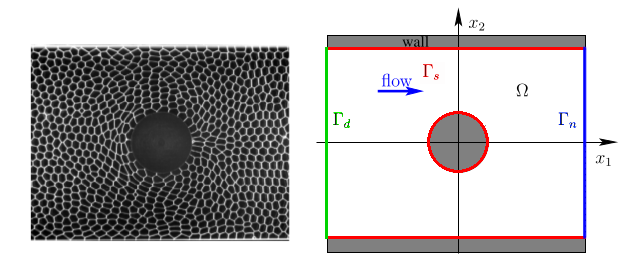
\includegraphics[scale=0.5]{domain.png}
\end{figure}

\end{frame}



\begin{frame}{Model}

\scriptsize
Find $\stress{\ \mathcal{U}} = (\Tau,\v, p)^T : \; \left]0,T\right[ \times \Omega \rightarrow \mathbb{R}^{d\times d} \times \mathbb{R}^d \times \mathbb{R}$ such that :

\vfill
$
   \left\{
       \begin{array}{l l l l}
           
           (1)& 
           W_e\left[\textcolor{blue}{\tensor{\od{\Tau}{t}}}\right] 
           + \textcolor{red}{\mathcal{K} \left( | \Tau_d | \right) \Tau} - 2\alpha \tensor{D(\v)}&
           =& 0_{\mathbb{R}^{d \times d}} \\
           
           \\

           (2)&
           R_e\left[ \pd{\v}{t} + 
           \textcolor{RoyalPurple}{\left(\v . \grad \right) \v} \right] 
           \underbrace{-\divv{\Tau -p\tensor{I}_d+2\eta_s\tensor{D(\v)}}}_{ -\divv{\Tau_{tot}} = -\divv{\Tau} + \grad p - (1-\alpha)\Delta\v}&
           =& 0_{\mathbb{R}^d} \\

           (3)& \div{\v} &=& 0_\mathbb{R} \\

           \\

           (4)& 
           \multicolumn{3}{l}{
           \v = \vector{v_{\Gamma_d}} \hskip 0.58cm \textrm{ in } ]0,T[\ \times\ \Gamma_d
           \hskip 2.4cm \v . \vector{n} = 0\textrm{ in } ]0,T[ \times \Gamma_s
           } \\
           
           (5)&
           \multicolumn{3}{l}{
           \vector{F} = \Tau \vector{n} = 0 \textrm{ in } \left]0,T\right[ \times \Gamma_n
           \hskip 0.9cm 
           \vector{F_t} = \Tau \vector{n} - \Tau_{nn} \vector{n} = 0 \textrm{ in } ]0,T[ \times \Gamma_s
           } \\

           (6)&
           \multicolumn{3}{l}{
           \Tau = \Tau_- \hskip 0.775cm \textrm{ in } \left]0,T\right[ \times \Gamma_-
           } \\
       \end{array}
   \right.
$
\vfill

\end{frame}


\begin{frame}{Operator Splitting}

\ssubtitle{We rewrite the model as:}
\scriptsize
\vskip 0.5cm

Find $\ \stress{\mathcal{U}} = (\Tau,\v, p)^T : \; \left]0,T\right[ \times \Omega \rightarrow \mathbb{R}^{d\times d} \times \mathbb{R}^d \times \mathbb{R}$ such that :

\vskip 0.3cm
\hskip 1.3cm
    $
    \left\{
        \begin{array}{l}
            \M \pd{\UU}{t} + \A{}{\UU}= 0_{\mathbb{R}^{d\times d}\times \mathbb{R}^d \times \mathbb{R}} &
            &
            (4) \hskip 0.5cm (5) \hskip 0.5cm (6) \hskip 0.5cm \textrm{(Boundary conditions)}
        \end{array}
    \right.
    $

        \vskip 0.5cm
\hskip 1.0cm with $\M =
    \left [
       \begin{array}{c c c}
           W_e&0&0&
           0&R_e&0&
           0&0&0&
       \end{array}
    \right ]
    \textrm{ and } \A{}{\UU} =  \alert{\A{1}{\UU}} + \textcolor{blue}{\A{2}{\UU}}
$

\vskip 0.5cm
$$
\A{}{\UU} = 
\underbrace{
    \left[\begin{array}{c}
            \textcolor{red}{\mathcal{K} \left( | \Tau_d | \right) \Tau} - 2\alpha \tensor{D(\v)}&
            -\divv{\Tau} + \grad p - (1-\alpha)\Delta\v&
            \div{\v}&
\end{array}\right]}_{\alert{\A{1}{\UU}}\ contains\ all\ \alert{viscoplastic\ effects}}
+
\underbrace{
    \left[\begin{array}{c}
           W_e\left[\textcolor{blue}{\left(\v . \grad \right) \Tau + \tensor{\beta_a \left( \Tau, \gradv \right)}}\right]&
           0&
           0&
\end{array}\right]}_{\textcolor{blue}{\A{2}{\UU}}\ contains\ all\ \textcolor{blue}{viscoelastic\ effects}}
$$

\end{frame}


\begin{frame}{$\Theta$-Scheme}

    \scriptsize
\ssubtitle{Three-steps $\theta$-scheme time-approximation of the previous equation :}

\vskip 0.5cm
Let $\Delta t > 0$ and $\theta \in \left] 0,1/2 \right[$ and $\UU_n$ be given. 
    
    \vskip 0.2cm
    \textbf{To compute } \textcolor{blue}{$\mathbf{\UU_{n+1}}$} \textbf{compute successively the following subproblems} :

    \tiny
$$
\begin{array}{l c c c l c l c r}
    \alert{\mathcal{P}_1}\left(\textcolor{blue}{\Uv},\Uu\right)&\Leftrightarrow&
    \M\dfrac{\textcolor{blue}{\Uv} - \Uu}{\theta \Delta t}&+&\A{1}{\textcolor{blue}{\Uv}}&+&\A{2}{\Uu}&=&0\\
    \\
    \alert{\mathcal{P}_2}\left(\textcolor{blue}{\Uw},\Uv\right)&\Leftrightarrow&
    \M\dfrac{\textcolor{blue}{\Uw} - \Uv}{(1-2\theta) \Delta t}&+&\A{1}{\Uv}&+&\A{2}{\textcolor{blue}{\Uw}}&=&0\\
    \\
    \alert{\mathcal{P}_1}\left(\textcolor{blue}{\Ux},\Uw\right)&\Leftrightarrow&
    \M\dfrac{\textcolor{blue}{\Ux} - \Uw}{\theta \Delta t}&+&\A{1}{\textcolor{blue}{\Ux}}&+&\A{2}{\Uw}&=&0
\end{array}
$$

\vskip 0.5cm
    \scriptsize
    \stress{The third step is similar to the first one.}


\end{frame}


%\begin{frame}{References}
    %\raggedright
    %\nocite{*}
    %\bibliographystyle{plain}
    %\bibliography{master}
    %\vfill
    %\begin{center}
        %\Large
        %Any questions ?
    %\end{center} 
%\end{frame}

\end{document}
